\documentclass[12pt]{article}

%\usepackage{hyperref}
\usepackage[hidelinks]{hyperref}
\usepackage[a4paper]{geometry}					
\usepackage[utf8]{inputenc}
\usepackage{lmodern,textcomp}
\usepackage{graphicx}

\usepackage[absolute,overlay]{textpos}
\usepackage{tikz}
\usetikzlibrary{arrows,positioning,shadows,shapes}
\usepackage{url}
% \usepackage{eurosym}
\usepackage{amstext}
\usepackage{caption}
\usepackage{subcaption}
\usepackage{listings}
\usepackage{float}
\usepackage{xcolor}

\geometry{hmargin={2.5cm,2.5cm},vmargin={2.5cm,2.5cm}} 	
\geometry{head=1.5cm, foot=1.5cm} 											

\pagestyle{myheadings}

\lstset{
  basicstyle=\ttfamily,
  breaklines=true,
  columns=fullflexible
}

\begin{document}
%------------------------- Title Page  -----------------------------------


\newcommand{\changefont}[3]{\fontfamily{#1} \fontseries{#2} \fontshape{#3} \selectfont}

% coordinates for the bg shape on the titlepage
\newcommand{\diameter}{20}
\newcommand{\xone}{-60}
\newcommand{\xtwo}{440}
\newcommand{\yone}{60}
\newcommand{\ytwo}{-700}


\begin{titlepage}
\setlength{\oddsidemargin}{1cm}
\setlength{\topmargin}{-1cm}


% bg shape
\begin{tikzpicture}[overlay]
\draw[color=gray]
   (\xone pt, \yone pt)
 -- (\xtwo pt, \yone pt)
arc (90:0:\diameter pt)
 -- (\xtwo + \diameter pt , \ytwo pt)
-- (\xone + \diameter pt , \ytwo pt)
arc (270:180:\diameter pt)
-- (\xone pt, \yone pt);
\end{tikzpicture}
\begin{textblock}{10}[0,0](1.5,1.3)
 
\includegraphics[width=.3\textwidth]{KITlogo.pdf}
\end{textblock}
\begin{textblock}{10}[0,0](8.3,1.3)
\begin{flushleft}
\large Institute f\"{u}r Technische Informatik\\
Chair for Embedded Systems
  \end{flushleft}
\end{textblock}

\changefont{phv}{m}{n} % helvetica
\vspace*{3.5cm}
{
\centering
 \huge{Design and Implementation of an IoT-based Control Device for an off-the-shelf Coffee Machine}

 \vspace*{2cm}
 \large{Bachelorarbeit \\
   von
 }\\
 \vspace*{1cm}
 \Large{Karim Ben Ammar}\\
 \vspace*{1cm}
 \normalsize{
 an der Fakult\"{a}t f\"{u}r Informatik\\
 }

\vspace*{3cm}
\normalsize{
\begin{tabular}[ht]{l c l}
   Betreuer: & \medskip  & Prof. Dr. J\"org Henkel\\
  %Betreuender Mitarbeiter: & \medskip & ...\\
   Betreuende Mitarbeiter : &\medskip & Dr.-Ing Lars Bauer \\
   Betreuende Mitarbeiter : &\medskip & M.Sc Farzad Samie \\
   Betreuende Mitarbeiter : &\medskip & M.Sc Marvin Damschen \\
 & & \\
 & & \\
%
%  Die nächsten 2 Punkte werden für Seminare nicht benötigt
%
  Tag der Anmeldung: & \medskip  & 31.1.2017\\
  Tag der Abgabe: & \medskip & 30.05.2017\\

\end{tabular}
}
%\begin{textblock}{10}[0,0](3,14)
%\large{Time: XX.04.2010 \hspace*{0.25cm} -- \hspace*{0.25cm} XX.XX.2009}
%\end{textblock}

}
%\begin{textblock}{10}[0,0](1.75,15.365)
%\tiny{
% KIT -- Universit\"{a}t des Landes Baden-W\"{u}rttemberg und nationales Forschungszentrum in der Helmholtz-Gemeinschaft
%}
%\end{textblock}

\begin{textblock}{10}[0,0](9.7,14.95)
Chair for Embedded Systems
 
\includegraphics[width=.07\textwidth]{CESlogo.pdf}
\end{textblock}


\end{titlepage} 

\clearpage
\begingroup
\pagestyle{empty}
\null
\newpage
\endgroup
\pagebreak
\topskip0pt
\vspace*{\fill}
\textbf{\LARGE{Selbstst\"andigkeitserkl\"arung}}
\bigbreak
\bigbreak
\bigbreak
\bigbreak
Ich versichere, dass ich die vorliegende Arbeit selbstständig angefertigt und
mich keiner fremden Hilfe bedient habe. Alle Stellen, die wörtlich oder
sinngemäß veröffentlichtem oder unveröffentlichtem Schrifttum entnommen
sind, habe ich als solche kenntlich gemacht.
\bigbreak
\bigbreak
\bigbreak
\bigbreak
\noindent\rule{\textwidth}{0.4pt}
Karlsruhe, 10.03.2020
\vspace*{\fill}
\clearpage
\begingroup
\pagestyle{empty}
\null
\newpage
\endgroup
\topskip0pt
\vspace*{\fill}
\begin{abstract}
  Wenn es zur Implementierung neuer und innovativer Technologien für bisher analoge Prozesse kommt,
  dann kann dies häufig zu einer tatsächlichen Verminderung der Benutzbarkeit für die Benutzer des Systems führen.
  Der offensichtliche Vorteil, eine Strichliste,
  die dazu verwendet wird Benutzer anhand ihres Kaffeekonsums aus einer handelsüblichen Kaffeemaschine,
  mit einem elektronischen, automatisierten System zu ersetzen, liegt darin, 
  die manuelle Arbeit des Schreibens und Zählens von Strichen zu sparen.
  Wenn das System allerdings derart unzuverlässig funktioniert,
  dass es einem Benutzer nicht mehr möglich ist die Kaffeemaschine zu verwenden,
  dann erfüllt die Implementierung eindeutig nicht die Erwartung, den Prozess für den Benutzer zu verbessern.
  In dieser Thesis wird eine bereits existierende IoT-basierte Anwendung, die zur Erfüllung der zuvor genannten Aufgabe entworfen wurde,
  untersucht und die mit deren Implementierung verbundenen Schwierigkeiten hervorgehoben,
  sowie die Verbesserungen beschrieben, die durchgeführt wurden um einen Punkt zu erreichen an dem die Benutzbarkeit des neuen Systems
  einen klaren Vorteil gegenüber der manuellen Ausführung der Aufgabe darstellt. 
\end{abstract}
\vspace*{\fill}
\begin{abstract}
  When it comes to implementing new and innovative technologies for previously analogue processes,
  often enough there is an actual decrease in usability for the users of the system.
  The most apparent benefit of replacing a tally sheet that is used to charge users according
  to their coffee consumption from an off-the-shelf coffee machine,
  with an electronic, automated system, lies in eliminating the manual work of writing and counting strikes.
  However, when the system operates unreliably, to such an extent that the user has no chance of using the coffee machine,
  the implementation clearly does not meet the expectations of improving the process for the user.
  Examining an existing IoT-based appliance that was designed for the before mentioned task,
  this thesis will highlight the difficulties of such an implementation and describe the
  improvements that were made to reach a point where the utilization of the new system
  is a clear advantage over performing the task manually.
\end{abstract}
\vspace*{\fill}
\pagebreak

\clearpage
\begingroup
\pagestyle{empty}
\null
\newpage
\endgroup
%-------------------------- Inhaltsverzeichnis ----------------------------
\tableofcontents
\thispagestyle{empty}
\pagebreak

\listoffigures
\clearpage
\begingroup
\pagestyle{empty}
\null
\newpage
\endgroup
\noindent
\textbf{ \LARGE{Acronyms}} \\~\\
\textbf{DBMS} Database Management System\\~\\
\textbf{DSI} Display Serial Interface\\~\\
\textbf{FSM} Finite-state machine\\~\\
\textbf{GPIO} General-purpose input/output\\~\\
\textbf{HTTP} Hypertext Transport Protocol \\~\\
\textbf{IPC} Inter Process Communication \\~\\
\textbf{IoT} Internet of Things \\~\\
\textbf{LAMP} Linux Apache MySQL PHP \\~\\
\textbf{NFC} Near Field Communication\\~\\
\textbf{PWM} Pulse Width Modulation \\~\\
\textbf{RFID} Radio-Frequency Identification\\~\\
\textbf{SPI} Serial Peripheral Interface\\~\\
\textbf{SoC} System on Chip \\~\\
\textbf{UID} Unique Identifier \\~\\
\clearpage
\begingroup
\pagestyle{empty}
\null
\newpage
\endgroup
%------------------------------ Hauptteil ---------------------------------

% \setcounter{page}{1}

\section{Introduction}
This thesis documents the improvements to an existing system that was designed to replace a tally sheet for coffee consumption.
The system is connected to an off-the-shelf coffee machine and
automates the registration of every coffee or hot water dispensed.

There are two systems that were used before\footnote{Cf. \cite{Thesis1} and \cite{Thesis2}.}.
For simplicity, in this text they will be named version 1 (V1) and version 2 (V2), respectively.
Version 3 (V3) is the resulting system with the improvements described in this thesis.
While version 1 reportedly has yielded very good results,
it had to be adjusted due to a change in the coffee machine model.
In V2, subsequently, the system was almost completely redesigned and rebuilt for the new coffee machine.
However, the developed design and implementation are incomplete and did not produce satisfying results.
There was an initial list of bugs and possible improvements for V2 and also newly requested features for V3.
Throughout the progress of this work, the list has been reiterated and further specified.
A final version of it, containing an analysis of all the previously known and newfound problems and shortcomings of V2,
can be found in \autoref{pa}.

This work aims to improve V2 by resolving all bugs and additionally increase its usability and reliability.
Making the transition as smooth as possible, without disruptions to the daily use, is a high priority.
In an attempt to reutilize as much of the design ideas and code of the previous works as possible,
the implementation evolved out of the code base of V2.
However, a large part of the existing components had to be redesigned and newly implemented.

In the ISO norm \cite{ISO:Usability}, \textbf{usability} is defined as the ``extent to which a system, product or service can be used by specified users to achieve specified goals with effectiveness, efficiency and satisfaction in a specified context of use."
In \autoref{sec:usability} this definition will be applied to evaluate the system.
Later it will be explained that \textbf{reliability}, in the sense of high availability and fault tolerance, is a direct consequence of the requirements for usability.
Put simply, the system has to be designed and implemented in a way that whenever a user wants to have a coffee or hot water,
the system is available and fully functional
and must never run into errors which inhibit the proper usage of the coffee machine.
Reliability also plays an important role in the \textbf{Internet of Things} (IoT) \cite{reliability}.
The concept of IoT can generally be described as the upgrade of formerly analog, offline devices and plainly physical objects, 
to highly interconnected, digital devices and is still one of the biggest trends in IT \cite{review,survey}.
% Its definitions vary but it is a very broad field incorporating ideas of ubiquitous and pervasive computing.
% and generally referred to as the \textbf{Internet of Things} (IoT). 
% The examined system might not strictly be an IoT appliance, 
% however the approach taken uses many of its ideas and key enablers.
% ---- maybe state why reliability
Although, the approach taken in the system examined here uses many of the key enablers of the IoT,
it can be argued that it does not fully deserve to be called an IoT appliance.
Missing key characteristics are, the inter-connectivity between multiple devices and systems,
the pervasiveness of all parts, i.e.,
the complete physical integration of the added hardware into the coffee machine,
and gathering data from sensors for later processing.
The distinction of ``IoT-based" is made here to indicate that the system uses
a combination of technologies which are considered IoT enablers and could easily serve 
as a foundation for an IoT appliance.
\begin{itemize}
  \item Access to a controlling server via HTTP
  \item NFC reading RFID tag attached to physical object (e.g. coffee mugs, key chain)
  \item Support for a mobile application\footnote{The mobile application will not be further examined in this thesis. Support for it was dropped in V3, as there were no users.}
  \item Reading sensor data
  \item High availability
\end{itemize}

In the next three parts of this thesis,
first an overview of background knowledge is given,
then the problems in V2 and their solutions in V3 are discussed,
and at the end a short conclusion will be drawn.

% There is only one POS-like device.
% Also it should be integrated with the coffee machine into one single device.

% Why improving and reliability Problem Analysis of Previous Work
%   The second one conducted a complete re-implementation of the first, 
%   which led to a degression in overall usability and reliability,
%   especially the code quality was poor. \textcolor{red}{TODO: specify}
%   IPC, GPIO, state machine described, not used, intransparent of states.

% maybe better transition to background


\section{Background}

\subsection{The Previous System (V2)}
The system, as it was used before this work started, included the following hardware components:
\begin{itemize} 
  \item Coffee machine Saeco Café Royal SUPE016RE
  \item Raspberry Pi 3 Model B v1.2
  \item Adapter board between the coffee machine and the Raspberry Pi
  \item RFID reader module by JoyIT, based on the NXP MFRC-522 frontend
  \item Buzzer connected to the Raspberry Pi
  \item 7" Touchscreen
  \item Ethernet cable
  \item Official Raspberry Pi micro-USB power adapter, 5.1V, 2.5A
  \item Shoe box, converted into a case for all components apart from the coffee machine
\end{itemize}

The coffee machine used, does not provide an interface to access its sensor data.
Therefore, in the previous works, an adapter board employing optocouplers
was designed in order to read and manipulate the coffee machine's internal sensors.
This was done by hijacking the cables coming from and going to the coffee machine's control board.
The three sensors available to the system now are:
\begin{itemize}
  \item \textbf{water flow:}
        The water flow through the coffee machine's pump is measured by a flow meter.
        The signal captured is a square wave signal, oscillating between logic high and low voltages.
        It has varying frequencies, dependant on water flow speed. A higher frequency implies more water output during a certain time interval.
        Time intervals vary in duration, since they depend on the user's preference for the amount of water.
        Note that while the current coffee machine has only one flow meter,
        the source code has support for two water flow signals.
        The reason is that the coffee machine model which was used before
        has two separate water circuits for coffee and hot water, i.e.,
        two separate signals available that help distinguish between coffee and hot water dispensing.
        With the new model, the adapter board did not change and the two different connectors still exist.
        However, both transmit the same input signal.

  \item \textbf{grinder:} The grinder signal is similar to the water flow signal, in that it is also a square wave signal.
        Interestingly, it can only be measured after the coffee machine has already finished grinding. 
        It then occurs for less than a second on average.
        Further analysis of the grinder signal is done in \autoref{sec:grinder}.
  \item \textbf{water level/blocking:} The water level signal is toggled every time
        the water contained in the fresh water tank sinks below a certain level.
        By intercepting the signal an empty water tank can be simulated to the coffee machine.
        This will effectively block the dispensing of water and coffee by putting the machine into ``no water mode".
        The system can leverage this mechanism to lock and unlock the coffee machine.
        However, the system then needs to inform the user when the water level is actually low,
        because the text on the coffee machine's display that says ``FILL WATERTANK" 
        will only indicate that the machine is locked and might be misleading otherwise.
\end{itemize} \label{itm:waterflow}

\subsubsection{The Raspberry Pi and GPIO}
The Raspberry Pi 3 Model B is a single-board computer integrating a Broadcom system on chip (SoC).
Its credit card sized form factor, numerous I/O capabilities, extensive documentation and the relatively cheap price of €35
are the reason why it is a popular choice for all kinds of maker projects and teaching.

The relevant parts of the specification for the Raspberry Pi model used are:
\begin{itemize}
  \item Broadcom BCM2837, quadcore Cortex-A53 (ARMv8) 64-bit SoC @ 1.2GHz
  \item 1GB LPDDR2 SDRAM
  \item 100 Base Ethernet
  \item Extended 40-pin GPIO header
  \item DSI display port for connecting a Raspberry Pi touchscreen display
  \item Micro SD port for loading your operating system and storing data
  \item 5V/2.5A DC power input
\end{itemize}
A complete specification can be found in the appendix \ref{PI:Spec}.

The general-purpose input/output (GPIO) header provides 40 input and output pins that each can be
configured and controlled independently by the user at run time.
The output voltage can be set to high and low. 
When set to high, the voltage has a minimum value of 3.0V and cannot be higher than 3.3V.
When set to low, the voltage has a maximum rating of 0.14V.
In input mode, gpio pins read voltages higher than 1.6V as high and voltages lower than 0.9V as low.
For each pin an interrupt can be set in the ARM, triggered by high/low levels or rising/falling edge.
There are also internal pull-up and pull-down resistors of $50 - 60 k\Omega$ that can be enabled optionally.
Furthermore, alternative functions can be assigned to the pins so they can be used for, e.g., PWM, I2C or SPI buses, and serial connections.
In total, the GPIO interface makes the Raspberry Pi highly versatile and opens up numerous possibilities
for connecting it to all kinds of periphery\footnote{See \cite{PI:GPIO} and \cite{PI:BCM} for a detailed description of the Raspberry Pi's GPIO capabilities.}.

The manufacturer of the Raspberry Pi provides Raspbian as the default operating system.
It is a Debian Linux derivative, especially designed for the Raspberry Pi.
It makes use of \texttt{systemd}, which, among other tasks, is in charge of managing system services.
Although many options exist, the de facto standard and best supported programming language for the Raspberry Pi is Python.
As a result, there are several libraries available for accessing the Raspberry Pi's GPIO from Python.
Three of the more important ones are:

\begin{itemize}
  \item \texttt{RPi.GPIO}, which is classically the most commonly used, but only offers basic functionality.
  \item \texttt{gpiozero}, which offers specialized high level objects representing different hardware components like buttons and LEDs,
        and is thus the easiest to use for simple tasks.
  \item \texttt{pigpio}, which is more sophisticated with a greater support for low level features like wave patterns,
        PWM and glitch/noise filters for edge detection.
        Unlike the other two, it runs as a system daemon that is accessed by clients via Unix sockets and also allows remote connections.
\end{itemize}

\subsubsection{Connection between Components}
A user authenticates with an RFID tag. The ID from the RFID tag is read by the RFID reader. 
The RFID reader is connected to the Raspberry Pi via the GPIO pins and is controlled using the SPI bus protocol.
After reading the ID, the system checks if there is a user in the database that registered with this ID.
If that is the case, the user will be logged in and the coffee machine will be unlocked.
The buzzer is used to give audible feedback when a user successfully logs in.

The touchscreen is directly plugged into the Raspberry Pi's Display Serial Interface (DSI).
Raspbian has built-in support for the screen and does not require special configuration,
allowing to use the provided desktop environment out-of-the-box.

The Raspberry Pi is connected to the local network through ethernet and also has internet access.
However, a stable connection cannot always be guaranteed.

Although, a case to contain all the components was designed in V2,
it was never finished, and thus the parts were assembled into a shoe box.

\subsubsection{Accounting Server}
The accounting server has a record of all registered users and their associated RFID tags.
It logs every order, every payment to recharge balance and
every withdrawal of money for consumables such as coffee beans and milk.
There is one person responsible for creating accounts,
registering RFIDs and entering withdrawals and recharges into the database.
Each user's current balance is calculated by summing up all withdrawal and recharge events from the past.
The events are kept in one large table in the database, whose history goes back to 2012.
This was the the year when the accounting server was created and that was before the work on V1 started.

The accounting server is accessed across the local network via an HTTP interface.\\
It operates on a typical LAMP stack.
A list of all registered users and their associated RFIDs can be obtained with:
\begin{lstlisting}
  http://i80web2.ira.uka.de/coffee/getusers.php?secret={some-secret}
  \end{lstlisting}
Information about a single user by RFID can be obtained with:
\begin{lstlisting}
  http://i80web2.itec.kit.edu/coffee/getuser.php?rfid={some-rfid}
  \end{lstlisting}
If there is a user associated to the given RFID, the response includes \texttt{user\_id}, \texttt{balance} and \texttt{token},
if there is no associated user, the response contains the string ``unknown token/rfid".
A \texttt{token} is an alphanumeric identifier for a user account. \\
An order is submitted to the accounting server with:
\begin{lstlisting}
  http://i80web2.itec.kit.edu/coffee/buy.php?rfid={some-rfid}&black={true/false}&water={true/false}&cheated={true/false}
  \end{lstlisting}

There is a graphical interface for direct access by users where they can see an overview of their consumption,
a list of every user's balance, activities like withdrawals and deposits to the treasury, and a ranking of ``good milk guys'' and ``bad milk guys''.
The latter are statistics based upon the ratio of milk brought to the office and milk consumed.

\subsection{Concurrency in Python, IPC and Multiprocessing}
Due to a mechanism in Python called Global Interpreter Lock (GIL),
in one python process only a single thread can execute at a time.
Other threads need to wait until the running thread releases the lock.
This limitation requires the usage of Python's \texttt{multiprocessing} library
to utilize more than one CPU core and run applications truly in parallel.
It allows to create processes with a similar interface as used for threading.

To communicate between these processes there are two types of channel integrated with the \texttt{multiprocessing} module.
\begin{itemize}
  \item Pipes and
  \item Queues
\end{itemize}

For direct communication between two processes, pipes are the simplest solution.
On Unix, pipes simply act as a higher level interface for sockets.
They open an either uni- or bidirectional connection between two processes,
returning a connection object that can be used to transmit data from one end to the other.
While sending or receiving on both ends at the same time is possible,
it will most certainly corrupt data when trying to send from more than one thread or process
on the same end of a pipe at the same time.
In other words, this implementation of pipes is not thread-safe.
However, queues offer a layer of abstraction, adding synchronized access on top of pipes
and hereby allow process- and thread-safe IPC.

Concurrency is also an important aspect of graphical user interface (GUI) programming.
If, e.g., a button press starts a long running calculation, the whole GUI would become irresponsible while the calculation is in progress.
Therefore, separate threads should be used for rendering the GUI and performing background tasks.
In Qt5, which is the GUI framework used in this work, there is the concept of slots and signals for thread safe asynchronous communication.
Signals with attached parameters can be emitted and will trigger the execution of connected slots, i.e., functions that accept the passed parameters.

\subsection{3D Printing}
For printing the 3D models that were designed in V2 and V3 the \textit{formlabs Form 2} 3D printer was used.
This printer uses the stereolithography (SLA) printing technique where a ``laser [is used] to cure solid isotropic parts from a liquid photopolymer resin" \cite{3dprinter}.
SLA belongs to the more expensive methods for 3D printing but therefore promises a much higher precision and resolution.
The printer has a resin tank with an elastic, transparent floor.
The tank is located on top of a glass window that shields the inner parts of the printer.
On the inside of the printer there is a stationary laser that is redirected into the resin tank 
by a high precision mirror system.
Since the laser has to pass the glass window and the floor of the resin tank, 
it reacts highly sensitive to impurities, such as dust and fingerprints, between these layers.
Refractions would impose potentially grave damage to printed models.
The model is growing layer by layer on the build platform, which is located above the resin tank and oriented upside down.
The platform is lowered into the resin tank for every new layer.
Whenever the platform sinks into the resin, it lightly pushes onto the elastic resin tank floor
to ensure only a thin layer of resin gets cured.
Unfortunately, this process causes the resin tank to wear out quickly. 
As a result, the resin tank has to be replaced after a printing volume from 1-1.5 liters of resin.

The 3D model was designed with the open source tool Blender.
Since Blender is a very advanced computer aided design tool,
where focus lies more on creating 3D models for animations,
it is hard for beginners to use it for 3D printing.
However, with the ``3D-Print Toolbox" add-on,
Blender offers tools for checking and repairing the designed models.

\subsection{Terms}
This is a description of the terms used in the context of this thesis.
\begin{description}
  \item [Order] An order is the selection of a coffee with milk, a coffee without milk, or hot water
        and always connected to a specific user.
  \item [Ordering Process] The process of placing an order that starts with
        the user authenticating and ends after the order was submitted to the accounting server.
  \item [System] The hardware and software that constitute the appliance.
    It includes the Raspberry Pi, the RFID reader, the buzzer, the amplifier circuit and all programs running on the Raspberry Pi.
    The accounting server and the coffee machine are explicitly excluded from this definition.
\end{description}

\section{Problem Analysis and Solutions}
\label{pa}

\subsection{Improving Usability}
\label{sec:usability}

In the introduction a definition of usability was given.
Starting by specifying the user, goal and context of use, and continuing with the requirements for effectiveness,
efficiency and satisfaction, the definition can be utilized as a guideline for evaluating the system.

\begin{description}
  \item [User]
        The majority of users are employees at the chair, i.e., the professor, post docs, the secretary, and research assistants.
        A small number of users are students either writing a thesis or working as assistants.
        Most users only use the coffee machine to order coffee. Hot water, however, is ordered very rarely.

  \item [Goal]
        % Use case 1: John wants to drink a coffee. He goes to the coffee machine, takes his token and holds it on the reader. 
        % His account is unlocked, now he can use the coffee machine to make coffee or hot water. He likes to drink his coffee with milk.
        % The system saved his preference for milk the last time and already has the "Add milk" option pre selected.
        % If John wants 
        The user's goal is to buy a coffee or hot water.
        The coffee can be with milk or without milk.
        The user adds milk manually and has to register their choice with the system.

  \item [Context]
        Users engage with the system in various situations, but usually only less than a minute.
        Some possible situations can be distinguished here:
        \begin{enumerate}
          \item The user is actively using the time to get a coffee as a short break.
          \item The user is in a conversation with a colleague.
          \item The user is marveling about a hard to solve work related problem.
        \end{enumerate}
        Furthermore, it has to be taken into account that the screen will likely be at a distance of more than 60cm from the user,
        which means that the font size should be significantly larger than the 11-points standard used in many operating systems. 
        It is also important to note that, because the screen is a touchscreen
        and interaction is haptic, there are certain constraints for the sizes of controls. 
        They have to be large enough to be easily usable.
        The time when users order coffee varies from day to day and cannot be specified in a fixed interval.
        Nevertheless, most orders occur between 10am and 6pm from Friday to Saturday.
        While it cannot be ruled out to receive an order at, e.g., 4am, it is very unlikely.


  \item [Effectiveness]
        The interactions with the system have to be leading towards the user's desired goal.
        If the interactions do not contribute to achieving the goal, the system is not effective.
  \item [Efficiency]
        There should be as few steps as possible required to achieve the goal.
        The total time needed for interaction with the system should be kept minimal.
  \item [Satisfaction]
        The user should be satisfied with the overall experience, have a positive attitude towards the system and feel comfortable using it. 
        Sources of frustration have to be eliminated.
        Satisfaction can be increased, for instance, with an appealing graphical design, the right use of colors and visuals, 
        but also by making it easy to learn how to use the system.
        That means visual and audible feedback should be used to guide the user through the ordering process to ultimately achieve the goal.

\end{description}

In summary, the system must not unnecessarily obstruct and distract the user and it must always focus on its main purpose, which is simplifying the tally sheet approach.
For the evaluation of V2 the list of problems and shortcomings is used.
The results are then taken into account for creating a new design for V3.

\subsection{Analysis of Problems and Shortcomings in the Previous System}
\label{pa:list}
There are several problems which have to be fixed and a few additional requirements that have to be met.

\begin{description}
\item [GUI01 Bad visibility of important information]
\label{pa:GUI01}
When the user logs in the only visual feedback is their name and balance appearing on the screen.
Furthermore, this information only takes up a small portion of the screen and is not in the center of attention.
The user can easily be unaware the changes on the screen, especially when distracted.
There is no explicit hint that the coffee machine is ready to use and the user has to guess, which makes first use unnecessarily difficult.
The entertainment content, which is irrelevant at the beginning of the ordering process, takes up most part of the available space on screen.
This is highlighted in \autoref{fig:order-view-v2}.
Applying the requirements for usability stated before, it becomes clear that this design is not ideal.

\item [GUI02 Milk preference controls to small]
\label{pa:GUI02}
It can be difficult for the user to select if they want a coffee with or without milk,
because the controls are only about 3.9mm in height on screen, and therefore, making it hard to tap them with the average fingertip.
When the user needs several attempts to set the milk choice, this is ineffective and can lead to frustration.

\begin{figure}[h]
  \centering
  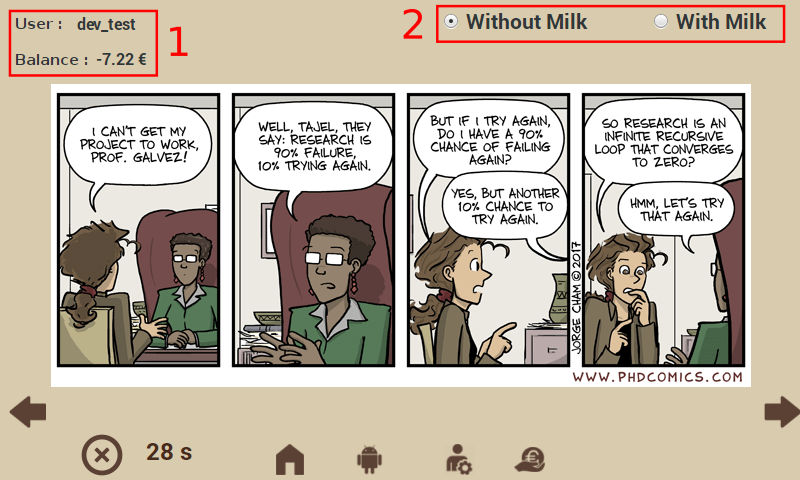
\includegraphics[width=\textwidth]{./images/order-page-v2.png}
  % \captionsetup{justification=left}
  \caption[Screenshot of the order view in V2.]
  {Screenshot of the order view in V2, taken from \cite{Thesis2}. \\
  1) The information displayed after a user successfully authenticated and the coffee machine is unlocked.\\
  2) The controls for selecting a milk option.}
  \label{fig:order-view-v2}
\end{figure}

\item [GUI03 Saving milk preferences not working]
\label{pa:GUI03}
The system should store if the user wants their coffee with or without milk.
Even though it was described as a feature in V2, the storage and retrieval of the preference was left unfinished.

Saving the milk preference increases efficiency by not prompting users for their milk choice on every order, saving them an additional interaction step.
Nevertheless, it has to be easy to change the preference during every order.


\item [GUI04 Entertainment content is not working]
\label{pa:GUI04}
Entertainment content (comics) is not shown anymore.
The script responsible for fetching content on the accounting server stopped working,
because of changes on the website(s) the content images were downloaded from.

The rationale behind showing entertainment content is to offer the user a form of engagement while waiting for the coffee machine to finish brewing.
If working properly, this feature can contribute to increase the overall user satisfaction.

\item [GUI05 Information for unknown RFID tag disappears to fast]\hspace*{\fill}
\label{pa:GUI05}
When a users tries to login with an unknown RFID tag a message is shown.
It informs about the necessary steps to take in order to use the coffee machine.
However, the message disappears after a very short time, making it difficult for the user to fully read it.
If the user removed their RFID card in the meantime, they have to place it on the RFID reader again to finish reading the message.
This is not effective.

\item [GUI06 Screensaver confuses users and fails to show if water is empty or not]
\label{pa:GUI06}
When the screensaver is activated, the screen turns completely black. 
The user cannot easily tell if the system is operating correctly or not.
Sometimes the screensaver does not deactivate when a user wants to order a coffee.
Especially, when the water tank is empty, there is no indication on the screen. This circumstance was found to confuse users.
From the usability point of view, this problem can frustrate the user or even stop them from accomplishing their goal,
i.e., using the coffee machine, and therefore must be avoided.

\item [BUG01 Coffee recognized as hot water]
\label{pa:BUG01}
When users order coffee, the system regularly fails to recognize it correctly and instead registers hot water.
This bug has the highest priority, since it can cause the treasury a financial deficit.

\item [BUG02 Rinsing after wake up charges the user with hot water]\hspace*{\fill}
\label{pa:BUG02}
After waking up from power save mode, the coffee machine might perform a rinsing.
The signal read by the system has the same characteristics as the signal for hot water.
Therefore, it is possible that the user is falsely charged for hot water.
A mechanism to detect this situation should be implemented.

\item [BUG03 The GUI freezes regularly, requiring a restart]\hspace*{\fill}
\label{pa:BUG03}
The GUI freezes from time to time, only showing a log-out button, but no logged-in user.
Measures should be taken that make it impossible for the GUI to freeze.
Again, if the GUI freezes, the system is not usable.

\item [BUG04 Free coffee when water tank is refilled]
\label{itm:BUG04}
When the water tank is refilled the coffee machine stays unlocked for about a second.
During this time frame a user could select a product without logging in and get coffee for free.
The system should only ever be unlocked when a user is signed in or maintenance mode is activated.

\item [BUG05 Free coffee when canceling while coffee is ground] \hspace*{\fill}
\label{itm:BUG05} 
When the user is logged in and selects coffee on the coffee machine.
The coffee machine starts grinding the coffee beans,
but the system only receives a signal after the grinding finished.
Before the grinding is recognized the user can press the cancel button and log out.
The coffee dispensing, however, will proceed without being registered by the system.
If the system recognizes a \texttt{coffee\_ground} signal without a user currently logged in, 
it should assume that, in case a user was logged in a few seconds before, it was them who ordered a coffee.
The system should register the coffee as a cheating attempt.

\item [BUG06 Offline mode not functional]
\label{pa:BUG06}
The system should be able to operate independently, without network connection, for a certain period of time.
The mechanism implemented in V2 is only partially functional.
The SQL query supposed to store offline orders in the database fails,
because it tries to insert data into non-existent columns.
Resolving this bug is of high priority for improving reliability.

\item [BUG07 RFID reader not responsive]
\label{pa:BUG07}
One of the challenges described in \cite{Thesis2} was that the RFID reader is not responding from time to time.
This problem still occurs.
The RFID reader is essential for using the coffee machine and has to work reliably.

\item [BUG08 3D-Model not printable]
\label{pa:BUG08}
In V2 a 3D model for a case to contain all the hardware was designed.
The model was split up into three components, the top, the bottom, and the screen frame,
to be able to fit into the 3D printer and later be assembled to form the case.
However, the screen frame was the only part that was completed and usable. The other two parts had design errors.
The bottom part was missing big enough holes for cables, the floor layer, with 1.28mm, was too thin and broke easily, and the walls, with 6.21mm, were very thick, and thus, wasting material.
The top part, which was supposed to sit on top of the bottom part and hold the screen frame,
was not printable due to floating planes and broken geometry, which can be seen in \autoref{fig:case-top-old}.
Even if it was printable, the design would have been problematic, because the RFID reader would have been located right in front of the screen,
resulting in cups with RFID tags attached, or big key chains blocking the view on the screen.
Furthermore, there were no structures to hold the Raspberry Pi or the RFID reader in place.

\begin{figure}[h]
\centering
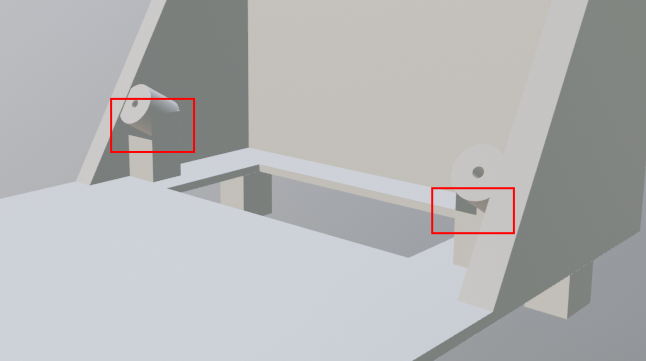
\includegraphics[width=\textwidth]{./images/case-top-annotated.png}
% \captionsetup{justification=centering}
\caption[Top part of the 3D model for V2.]
{Top part of the 3D model for V2.
Broken geometry that made the model unprintable is highlighted.}
\label{fig:case-top-old}
\end{figure}

\item [F01 No support for new KIT-Card]
\label{pa:F01}
A common way to authenticate with the device is to use the NFC-enabled KIT-Card\footnote{
  Every employee and every student at KIT has a KIT-Card.
  It is used, for example, as an access key to buildings, to rent books at the library
  and to pay meals in the canteen.}.
Throughout the past year all KIT-Cards were replaced by a newer model,
which uses the MIFARE DESFire EV1 integrated circuit for NFC.
The new model should be supported in V3.

\item [F02 High CPU usage]
\label{pa:F02}
During normal operation with no user interaction one core of the CPU
is constantly at around 95+\% utilization\footnote{Performance measurements of V2 can be found in \autoref{tab:perf-v2}.}.
This load appears to be very high when taking the available processing power into account.
The problem lies in how the sensor data is read from the coffee machine.
The signals are read and processed inefficiently at a frequency of 1kHz.
See an excerpt of the code in \autoref{code:v2}.
The load should be reduced to save power and avoid negative effects on hardware health.

\item [F03 Warm-up requires the user to log in several times]\hspace*{\fill}
\label{pa:F03}
The session expires 90 seconds after login.
This time interval is not long enough to warm up the coffee machine after a long idle time, e.g., after being idle over night.
Heating time, according to the manual, is approximately 2 minutes.

\item [F04 Logging not sufficient]
\label{pa:F04}
The existing logging system prints messages to the console and several log files.
However, the information is not clear, often missing information about its origin and timestamp.
This makes it very difficult to reason about the possible causes of a problem.
The system should have a proper logging mechanism to allow better debugging,
easy locating of errors and thereby improve the overall reliability.

\item [F05 Text files are used for IPC]%\hspace*{\fill}
\label{pa:F05}
Reasoning that the performance of pipes or sockets is not sufficient for IPC \cite[3.3.5]{Thesis2},
V2 uses simple text files in the working directory for communicating between processes.
An example of it can be seen in \autoref{code:v2}.
The arguments made against pipes that ``due to the different processes cycles, this solution was slowing the system"
and sockets ``blocking solutions will stop the system'', do not convince.
Especially, because using text files in the filesystem is essentially the same as using named pipes in Unix
with the disadvantage of being unmanaged by the kernel and causing unnecessary writes to the flash drive.
In total, the way IPC is implemented here, makes communication between processes opaque and difficult to reason about.

\item [F06 Buzzer has only one sound]
\label{pa:F06}
For a richer user experience and better audiovisual feedback, more sounds should be available.

\item [F07 The system has poor code quality that makes it hard to maintain]\hspace*{\fill}
\label{pa:F07}
Code is mostly undocumented, function and variable names are not always chosen meaningfully.
Compare \autoref{code:v2}.

\begin{figure}[H]
\centering
\begin{lstlisting}[language=Python, basicstyle=\footnotesize, frame=single]
def printLog(array):
    ...
    if not os.path.isfile("/home/pi/CoffeeMachine/UI/maintenance.txt"):
        global previousGrinder
        if GPIO.input(grinderPin) == 0 and previousGrinder == 1 and not currentOrder == 'coffee':
            if os.path.isfile("/home/pi/CoffeeMachine/UI/order.txt") :
                with open("/home/pi/CoffeeMachine/UI/order.txt", "r") as j:
                    temp = j.readline()
                if temp == "water\n":
                    os.remove("/home/pi/CoffeeMachine/UI/order.txt")
            with open("/home/pi/CoffeeMachine/UI/order.txt", "a+") as f:
                f.write("coffee\n")
                f.close()
            with open("/home/pi/CoffeeMachine/UI/stop.txt", "a") as f:
                pass
            currentOrder = 'coffee'
            previousGrinder = 1
        elif GPIO.input(grinderPin) == 1 and previousGrinder == 0:
            previousGrinder = 1
        elif not (GPIO.input(waterFlow1Pin) == previousWaterFLow1) or not (GPIO.input(waterFlow2Pin) == previousWaterFLow2):
            previousWaterFLow2 = GPIO.input(waterFlow2Pin)
            previousWaterFLow1 = GPIO.input(waterFlow1Pin)
            idleCount = 0
            if not os.path.isfile("/home/pi/CoffeeMachine/UI/order.txt"):
                with open("/home/pi/CoffeeMachine/UI/order.txt", "a+") as f:
                    f.write("water\n")
                currentOrder = 'water'
            elif not os.path.isfile("/home/pi/CoffeeMachine/UI/unlock.txt") and os.path.isfile("/home/pi/CoffeeMachine/UI/order.txt") and currentOrder == 'water':
                with open("/home/pi/CoffeeMachine/UI/unlock.txt", "a") as f:
                    pass
\end{lstlisting}
\caption[Code excerpt from V2's \texttt{inputGPIO.py}.]
{Code excerpt from V2's \texttt{inputGPIO.py}. The name of the function is misleading.
  Here the \texttt{coffee\_ground} and \texttt{water\_flow} signals are detected,
  then the type of order is determined and at last unlocking of the coffee machine is initiated.
  The function is run in a loop with 1ms sleep after each execution.}
\label{code:v2}
\end{figure}

\end{description}

\subsection{Design and Implementation of a New Solution (V3)}
In the previous section the flaws of V2 become clear.
Here the measures taken for improvement in V3 will be elaborated.
\subsubsection{System Architecture}
The finite state machine (FSM) is the core logic component of the system
and is in charge of the control flow.
There are eight possible states the FSM can be in.
The states are mapped to the steps of the ordering process.
Signals read from the coffee machine can trigger the defined state transitions.
As a result of the circumstances explained in  \autoref{itm:waterflow}, the transitions \texttt{flow\_1\_started} and \texttt{flow\_2\_started} are triggered by the same signal, 
as are \texttt{flow\_1\_stopped} and \texttt{flow\_2\_stopped}. 

\begin{figure}[h]
  \centering
  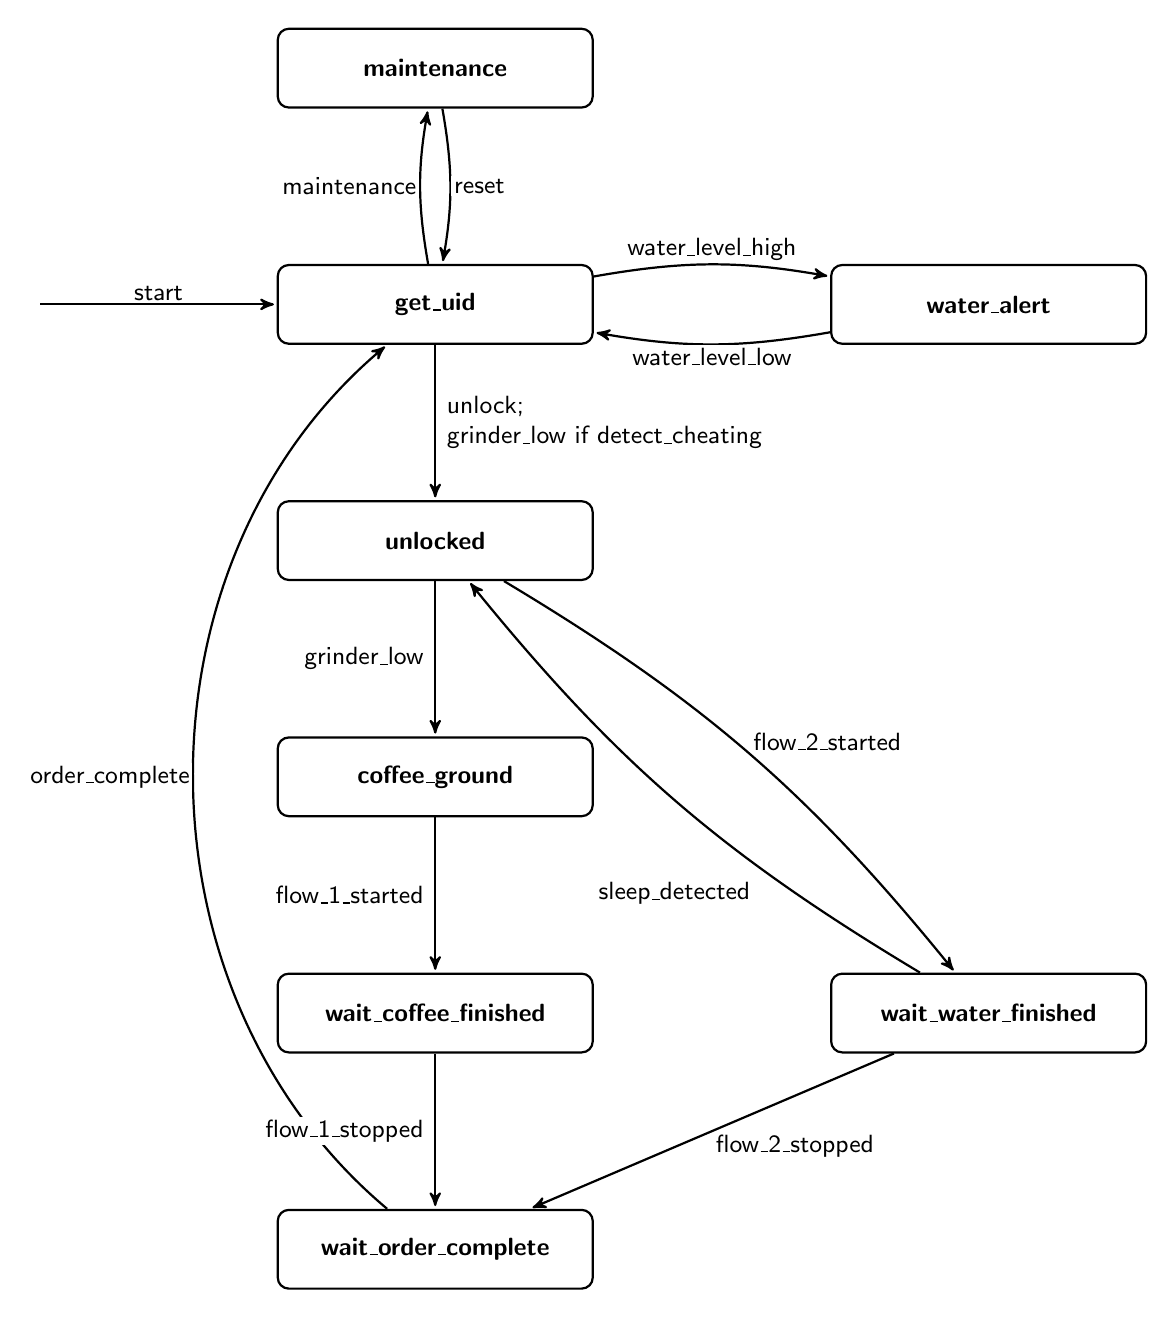
\begin{tikzpicture}[->,>=stealth',shorten >=1pt,auto,node distance=3cm,
      thick,main node/.style={rectangle,rounded corners,draw,
          font=\sffamily\small\bfseries,minimum width=40mm,minimum height=10mm},
      empty node/.style={inner sep=0, outer sep=0}]

    \node[main node] (mtn) {maintenance};
    \node[main node] (gu) [below of=mtn] {get\_uid};
    \node[main node] (wa) [right=of gu] {water\_alert};
    \node[main node] (ul) [below of=gu] {unlocked};
    \node[main node] (cg) [below of=ul] {coffee\_ground};
    \node[main node] (wcf) [below of=cg] {wait\_coffee\_finished};
    \node[main node] (wwf) [right=of wcf] {wait\_water\_finished};
    \node[main node] (woc) [below of=wcf] {wait\_order\_complete};
    \node[empty node] (start) [left=of gu] {};

    \path[every node/.style={font=\sffamily\small,
          fill=white,inner sep=1pt}]
    %   % Right-hand-side arrows rendered from top to bottom to
    %   % achieve proper rendering of labels over arrows.
    %   (M) edge [loop above] node {PrRd/-, PrWr/-} (M)
    (start) edge node {start} (gu)

    (wa) edge [bend left=10] node {water\_level\_low} (gu)


    (ul) 
    edge [] node[left=1mm] {grinder\_low} (cg)
    edge [bend left=10, yshift=-3pt] node {flow\_2\_started} (wwf)

    (woc) edge [bend left=50] node {order\_complete} (gu)
    (cg) edge [] node[left=1mm] {flow\_1\_started} (wcf)
    (wcf) edge [] node[left=1mm] {flow\_1\_stopped} (woc)

    (wwf) edge [] node {flow\_2\_stopped} (woc)
    edge [bend left=10] node[right=2mm,below=10mm] {sleep\_detected} (ul)

    (gu) edge [bend left=10] node {water\_level\_high} (wa)
    edge [bend left=10] node {maintenance} (mtn)
    %  edge [] node[left=1mm] {unlock} node[right=1mm] {grinder\_low if detect\_cheating} (ul)
    edge [] node[right=1mm, align=left] {unlock; \\ grinder\_low if detect\_cheating} node[right=1mm] {} (ul)

    (mtn) edge [bend left=10] node {reset} (gu)
    ;

  \end{tikzpicture}
  \caption[The finite state machine.]{The finite state machine. It is the core logic component of the system.}
\end{figure}
The existing states are:
\begin{description}
  \item [get\_uid] The RFID reader continuously tries to read an RFID from a card or tag.
        If an RFID is read the system will try to retrieve an associated user account, if possible\footnote{The network connection could be down. See \autoref{sec:offline-mode}}, from the accounting server, otherwise from the local database.
        If there is an associated user for the given RFID, the unlock transition will be triggered, if not, a message will be displayed,
        explaining to the user how to create an account.
        While in this state, the GUI will display entertainment content.

  \item [unlocked] The coffee machine is unlocked by unblocking the \texttt{water\_level} signal.
        The user is now able to use the coffee machine to order coffee or hot water.
        The touchscreen will now display the user's name, balance and last order.
        Also the milk preference, which was stored from the last order, is now preset.
        The user can change it until reaching the state \texttt{wait\_order\_complete}.

  \item [wait\_water\_finished]
        \label{itm:bug01}
        The \texttt{flow\_2\_started} event was detected, signalling the start of hot water dispensing.
        On the touchscreen the user can now see the choice made. Because of the problems with the sensors described before in \textbf{BUG01} and later in \autoref{sec:grinder},
        the GUI will ask the user for confirmation if they really ordered water. The question can be answered with ``Yes" or ``No".
        The default is to assume that the user wanted coffee, because a false positive of water inflicts a direct financial loss.
        If ``Yes" is selected the order will count as hot water. If ``No" is selected the order will count as coffee and
        the user has the option to toggle the milk choice button.

        After a certain time without use, the coffee machine will enter \textit{power save mode}, also referred to as sleep.
        The idle time before sleep can be set in the coffee machine's menu \cite{Saeco}.
        Currently, it is set to 3 hours.
        To leave power save mode, the coffee machine's menu button has to be pressed.
        The coffee machine will now warm up for about 2 minutes, depending on ambient temperature, and may or may not perform a rinsing afterwards.
        The system has to distinguish between a valid rinsing and a user ordering hot water.
        Therefore, it needs to detect if the coffee machine was in power save mode.
        This is done by checking for the last time an order was submitted, whenever entering the \texttt{wait\_water\_finished} state.
        If the last order was more than 3 hours ago,
        assume the coffee machine was in power save mode and trigger the \texttt{sleep\_detected} transition.

  \item [coffee\_ground]
        The \texttt{grinder\_low} signal was detected. It is certain now that the user ordered coffee.
        The system will remain in this state until the water flow starts.

  \item [wait\_coffee\_finished]
        The \texttt{flow\_1\_started} event was detected, signalling the start of coffee dispensing.
        If the user presses the ``OK" button, 
        the entertainment content will be shown and a note that the system will be ready for a new order in a few moments.
        At the same time the transition to \texttt{wait\_order\_complete} is initiated.

  \item [wait\_order\_complete]
        Once reached this state, the system offers the user one last chance to change the milk choice.
        The user can confirm the order by pressing the ``OK" button and will be presented with the entertainment content while waiting for the dispensing to finish.
        The order will only be completed and passed to the accounting server after the dispensing finished and an additional timer of 20 seconds ends.
        With the timer in place the user can still view their order and reconsider their milk choice after coffee was dispensed.

  \item [maintenance]
        Maintenance mode was activated by a user who entered the passcode to access the admin menu.
        In this mode the coffee machine is unlocked and sensors are ignored.
        The state can be reset to \texttt{get\_uid} from the admin menu.

  \item [water\_alert]
        This state is entered when the \texttt{water\_level\_high} event was detected.
        The naming refers to the logic signal from the coffee machine that switches to high when the water level in the water tank is low.
        Although, the signal could be toggled while dispensing coffee,
        the only valid transition can be started from the \texttt{get\_uid} state.
        Still, it is important to enter the \texttt{water\_alert} state after the ordering process completed,
        otherwise users would not get informed about the empty water tank.
        To keep the FSM simple, a flag variable was used instead of modeling additional states.
        The flag is set and reset whenever the signal is toggled.
        If the flag is set on entering \texttt{get\_uid}, the transition to the \texttt{water\_alert} state is made immediately.


\end{description}


\subsubsection{Process Organization and IPC}
Because the system has to render the GUI, read from the RFID reader and the coffee machine's sensors and play a sound on the buzzer almost at the same time.
it improves performance and responsiveness when these tasks are split up into several processes.
Due to the limitations of Python, using threading would not be an option here.
For communication between processes, Python's Pipes are used and replace text file method described in \textbf{F05}.
With the pipes a bi-directional connection between every subprocess and the main process, as is depicted in \autoref{fig:ipc}, is established.
There is a predefined set of messages in \texttt{util.py}.
The messages are further separated into the two types ``CMD", for command and ``E", for event.
Generally, if the message is a command, this indicates that it is sent by the main process and received by the subprocess.
Events, on the other hand, are received by the main process and sent by the subprocess, potentially triggering a state transition in the FSM.

\begin{figure}[!h]
  \centering
  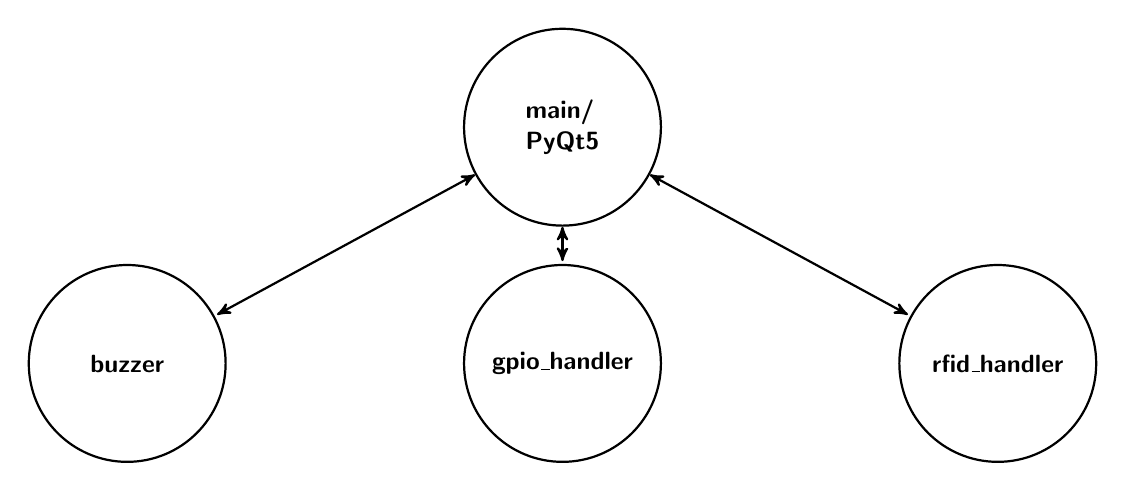
\begin{tikzpicture}[<->,>=stealth',shorten >=1pt,auto,node distance=3cm,
      thick,main node/.style={circle,draw,
          font=\sffamily\small\bfseries,minimum width=25mm,minimum height=10mm},
      empty node/.style={inner sep=0, outer sep=0}]

    \node[main node, align=left] (main) {main/ \\ PyQt5};
    \node[main node] (gpio) [below of=main] {gpio\_handler};
    \node[main node] (rfid) [right=of gpio] {rfid\_handler};
    \node[main node] (buzzer) [left=of gpio] {buzzer};

    \path[every node/.style={font=\sffamily\small,
          fill=white,inner sep=1pt}]
    %   % Right-hand-side arrows rendered from top to bottom to
    %   % achieve proper rendering of labels over arrows.
    %   (M) edge [loop above] node {PrRd/-, PrWr/-} (M)
    (main) edge [] node {} (gpio)
    edge [] node[left=1mm] {} node[right=1mm] {} (rfid)
    edge [] node {} (buzzer);

  \end{tikzpicture}
  \caption{Relation between the four processes.}
  \label{fig:ipc}
\end{figure}

Messages shared by all subprocesses:
\begin{itemize}
  \item CMD\_PAUSE: Pause execution of subprocess until CMD\_RESUME is received.
  \item CMD\_RESUME: Resume execution of subprocess.
\end{itemize}

Messages specific to GPIOHandler:
\begin{itemize}
  \item CMD\_LOCK: Lock coffee machine.
  \item CMD\_UNLOCK: Unlock coffee machine.
  \item E\_FLOW\_1\_STARTED: The start of flow meter 1 was detected.
  \item E\_FLOW\_1\_STOPPED: The stop of flow meter 1 was detected.
  \item E\_FLOW\_2\_STARTED: The start of flow meter 2 was detected.
  \item E\_FLOW\_2\_STOPPED: The stop of flow meter 2 was detected.
  \item E\_WATER\_LEVEL\_HIGH: The water level signal was triggered to high.
  \item E\_WATER\_LEVEL\_LOW: The water level signal was triggered to low.
  \item E\_GRINDER\_LOW: The grinder signal was triggered to low.
\end{itemize}
Messages specific to RFIDHandler:
\begin{itemize}
  \item E\_GOT\_ID: Signal that a user id was read.
        It has to be directly followed by a message string containing the id just read.
\end{itemize}
Messages specific to Buzzer:
\begin{itemize}
  \item CMD\_BUZZ: Make buzzing sound.
\end{itemize}

The ability to pause and resume the execution of processes
contributes to a lower resource usage.
The RFID reader is not required to check for new RFIDs once a valid RFID was read,
so the process can sleep while the FSM is not in the \texttt{get\_uid} state.

The processes are now managed as a \texttt{systemd service}. It replaces \texttt{Cron}, which is another service on Linux systems to allow scheduling tasks.
Unlike \texttt{cron}, \texttt{systemd} automatically detects crashes and can initiate a restart.
Furthermore it allows easy stopping and restarting of services, and the program's console output is automatically redirected to syslog. 
The configuration file can be found in the appendix \ref{systemd-service}.

\subsubsection{Logging}
The insufficiencies of V2's logging system are described in \textbf{F04}.
Because of the importance for debugging, the logging system was the first topic worked on.
It is indispensable for identifying the causes when encountering errors and receiving bug reports.
Python offers great support for logging with the \texttt{logging} module from its standard library. 
To meet the requirements of this software it was adjusted to achieve that:
Different log levels can be set for each imported module individually;
Every log entry has the source module attached to it;
Every log entry has the exact timestamp attached to it;
All the logs are redirected to Raspbian's \texttt{syslog} and thus can be easily searched with standard tools.
The operating system will also take care of automatically rotating logs, archiving and eventually deleting old entries.
Additionally, having all the logs in one single place, makes following the timeline of events when debugging a lot easier.

\subsubsection{The New GUI Design}
Taking into account the problems described in \ref{pa:list},
the GUI was redesigned with a focus on usability.
% Colors were used to enhance 
To address \textbf{GUI01}, elements in the GUI such as the current user name,
balance and milk choice were reorganized to center focus on them.
Additionally, the exact time, the product choice and the price of the last order were added to the view.
This information is not only ``nice to have", but also helped with finding errors,
since it allowed users to easily check if their last order was registered correctly.
The entertainment content will only be shown before the user logs in and then again after the ordering process ends.
To make it easier for first-time users, every step of the ordering process will cause visual feedback on the screen.
When a user successfully logged in they will see a confirmation that the coffee machine was unlocked.
The milk preference is already loaded and can be changed now or after selecting a product on the coffee machine.
At this point the user can still cancel the order by pressing the "Cancel" button.

The timeout after login that was causing problem \textbf{F03} was increased to 3 minutes and thereby adds a 1 minute buffer on top of the approximate heating time.
Furthermore, it is reset every time the screen is touched. Like this, the user will not have to log in several times while the coffee machine is heating. 

To solve \textbf{GUI02}, the size of all buttons was increased to at least 21.68mm in height and width,
which is large enough to easily tap them. This change increases effectivity and decreases frustration that occurred when more than one try was needed to change the milk choice.
By using the standard style for buttons they have a familiar look and are easily recognizable as such.
This is especially an improvement towards using only icons that do not look like they are clickable/touchable, as it was done in V2.

Once the product choice is recognized, 
the user will see both a symbolic and a textual representation of the order.
The symbolic representation is either coffee beans or water drops, and a crossed out or checked milk container depending on milk choice.
The textual representation is a summary of the order, showing the choice and total price. See \autoref{fig:gui-new-2}.

Freezing of the GUI, as described in \textbf{BUG03},
was found to be the result of the system being trapped in one or more undefined situations that occurred in edge cases.
As a side effect from the implementation of the state machine in V3 these problems now can be ruled out.

% After selecting the product the user can, but does not have to, confirm the order.
% It happens automatically after a timeout of 10 seconds. efficiency
In order to resolve \textbf{GUI06}, the screen saver was deactivated permanently.


\begin{figure}[h]
\centering
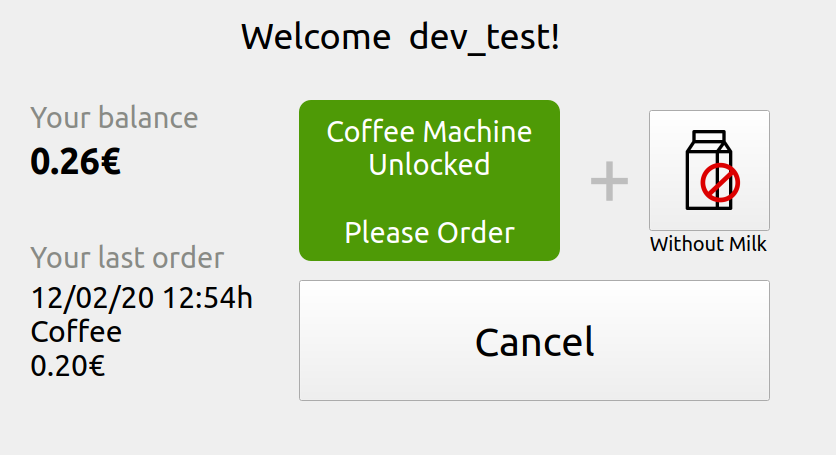
\includegraphics[width=\textwidth]{./images/gui-new-1.png}
\caption{The GUI when the user successfully logged in.}
\label{fig:gui-new-1}
\end{figure}
\begin{figure}[h]
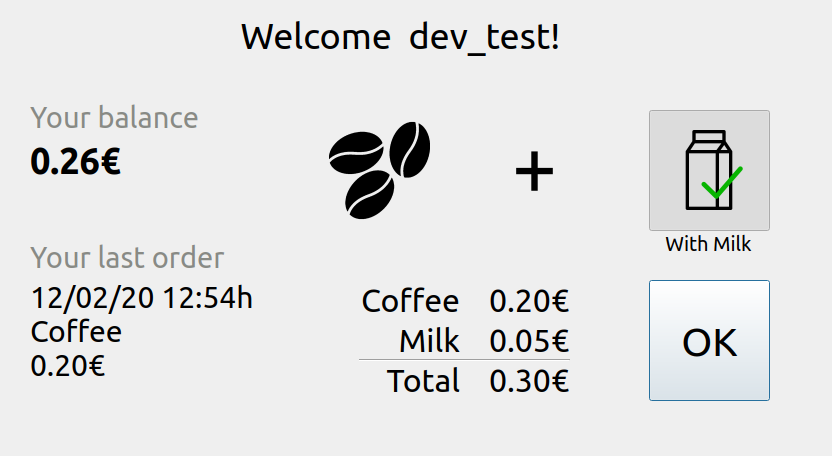
\includegraphics[width=\textwidth]{./images/gui-new-2.png}
\caption[The GUI after the user selected coffee on the coffee machine.]
{The GUI after the user selected coffee on the coffee machine. The ``With Milk" button was toggled to add milk to the order.}
\label{fig:gui-new-2}
\end{figure}

\subsubsection{Dispensing Limit}
By setting a dispensing limit, users are encouraged to pay their debts earlier.
The dispensing limit is reached when the balance of an account falls below a certain threshold.
There are two stages, which can be configured individually.
The first stage is merely a warning that is displayed in 
the GUI every time a user logs in, right before selecting a product.
But once the second stage is reached,
the user will not be able to unlock the coffee machine without recharging their account balance before.
Instructions on how to recharge their balance are shown to the users in this case, too.

Although a mechanism limiting dispensing like this existed in V1,
there is no sign of an implementation or description of such a mechanism in V2.

The accounting server has basic support for such a mechanism but there is no properly designed interface\footnote{The current state for each user would have to be parsed from the different colors and text in an HTML document.} to access the information.
Because changes to the accounting server are meant to be kept minimal, the better solution was to implement a standalone mechanism on the Raspberry Pi.
In the appendix \ref{app:dispensing} there is an explanation on how to set the thresholds for the two stages.

\subsubsection{Replacing the Buzzer}
The previously used buzzer was replaced by one of a different type to allow varying tones to be played (\textbf{F06}).
The new buzzer mainly consists of a piezo christal that moves to either one position when it is pulled to high or low.
One can hear a single clicking sound when the input changes from low to high.
Now, by applying a square wave input signal with a frequency in the audible spectrum - and the spectrum permitted by the buzzer's physical constraints - a single note can be played.
For example, switching the signal on and off with a frequency of 440Hz results in the note A4 being played.
A frequency of 220Hz would result in an A3, 880Hz would be an A5.
Since the wave signal is synthesized in software, occasional deviances of sound depending on processor load will occur.

At first, the new buzzer's volume was not satisfactory when directly attached to the Raspberry Pi's GPIO output,
because the Raspberry Pi's GPIO output voltage is 3.3V at maximum.
Increasing the buzzer's input voltage directly results in a higher volume.
Therefore, in order to get a higher volume,
it was sufficient to create a CMOS circuit for switching the 5V available from the Raspberry Pi's power lane as the buzzer's input voltage.
There is a schematic of the amplifier circuit in \autoref{fig:buzzer-amplifier}.
\begin{figure}[h]
  \centering
  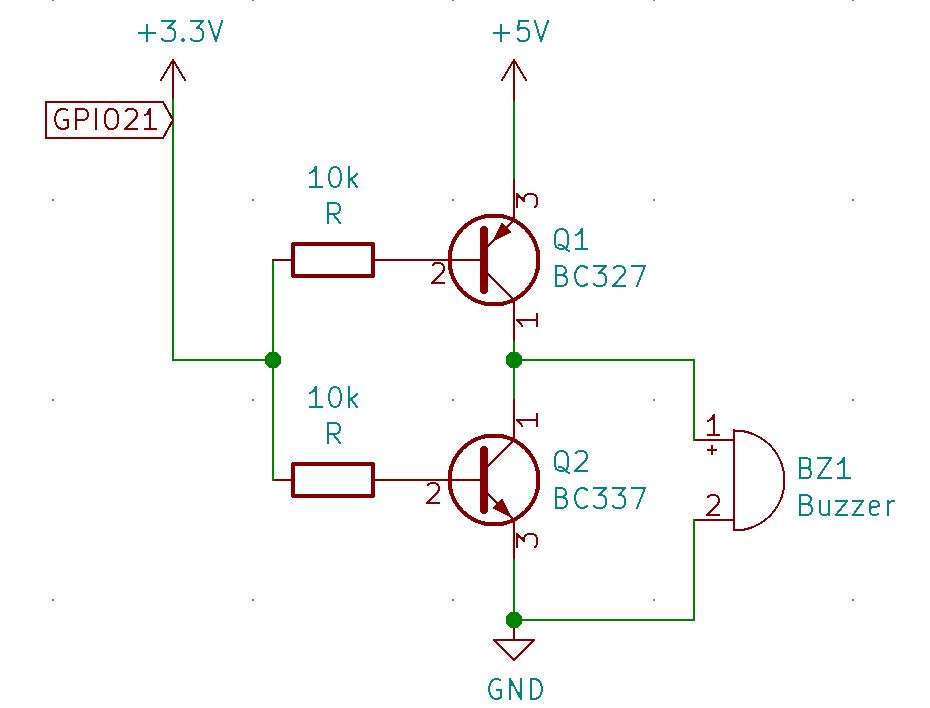
\includegraphics[width=15cm]{./images/buzzer-schema.png}
  % \captionsetup{justification=centering}
  \caption{Schematic of the amplifier built for the buzzer.}
  \label{fig:buzzer-amplifier}
\end{figure}

The new sounds for login and logout are a low tone followed by a high tone for login and a high tone followed by a low tone for logout.
The logout sound is also used for signalling that the water tank was successfully refilled.
When the account is locked, because of the dispensing limit a special sound is played.

\subsubsection{Debugging the RFID Reader}
With the help of the logging system the problems with the RFID reader, described in \textbf{BUG07},
could be narrowed down to be related to the software library, \texttt{mfrc522}, used for connecting to the device.
The logs proofed that all other parts of the system were executing as expected. 
Especially, the loop in which the code for accessing the library was ran every half second, always returned without an error,
invalidating the initial theory that the process was killed or blocking at some point.
This led to the key observation that after reinitializing the library, the reader was fully functional again.
Consequently, the simplest solution was to use a timer to completely reinitialize the RFID reader every five minutes.
Further investigation into the topic could start with the ``power reduction modes", which are mentioned in the modules data sheet \cite{MFRC522:doc}.

The KIT-Card issue \textbf{F01} was resolved by simply updating the library.


\subsubsection{Changes in GPIO Handling}
\label{sec:cpu-usage}
To reduce the high CPU usage mentioned in \textbf{F02},
the method to read the GPIO signals was changed.
Instead of polling at a sample rate of 1kHz in less performant Python code,
the responsibility for polling was completely moved to the GPIO library.
By setting up interrupts to trigger callbacks,
hardware capabilities for polling can be leveraged and, in consequence, significantly reduce CPU usage.
In the process of rewriting GPIO handling, RPi.GPIO was replaced by pigpio.

After implementing the logging system an important observation was that the \\
\texttt{water\_alert} and \texttt{coffee\_ground} events were triggered seemingly at random, without relation to any user interaction.
Sometimes an event could be triggered by switching the light off and on again in the same room the system is set up.
This indicates a high sensitivity to noise from the power supply.
% and on the other hand suggests a fault in the adapter circuit that connects the coffee machine and the Raspberry Pi.
% \textcolor{red}{TODO: why?}
To avoid problems caused by falsely recognized signals, a glitch filter was applied to every signal read from the machine.
The glitch filter effectively filters noise from signals by only toggling the signal if the input was in a stable state for a fixed period of time.
Measurements were performed throughout a month to determine a suitable parameter for the filter.
Switching the GPIO library from RPi.GPIO to pigpio, made using a glitch filter an easy task, as it already comes implemented with pigpio and can be activated optionally.
The parameters for the signals were set to 3500µs for water\_flow, 10000µs for water\_level and 30µs for grinder.
The values were determined by measuring and observing each signal.
% It proved to be a good heuristic to take the 
% \textcolor{red}{TODO: häufigkeitsverteilung}
The sample rate of pigpio is set to 200kHz, i.e., a signal is polled every 5µs.
Signals with a lower resolution than that will not be recognized.

\label{sec:grinder}
Sometimes the grinder signal is not recognized, which is one of the reasons that \textbf{BUG01} occurred.
The noise filter as a possible cause for the bug could be ruled out after measuring the signal with the filter deactivated.
Keeping in mind that the lowest resolution signal that gets recognized has a period length of 10µs,
and that typical period lengths for the coffee ground signal are about 100µs, it seems very unlikely that a too low sample rate could be the problem. 
Unfortunately, the exact reason for this problem could not be found 
nor explained by software related issues.
Which leaves a fault in the adapter board as the most probable cause for the problem.

% Therefore, the special handling of hot water dispensing was implemented. in the \texttt{wait\_water\_finished}.

\subsubsection{Operation in Offline Mode}
\label{sec:offline-mode}

To reflect \textbf{BUG06}, the system was designed with possible network outages in mind.
So when the accounting server cannot be reached, a user is still able to use the coffee machine.
Furthermore, the system will handle network errors gracefully and will not crash.

For the offline mode a local copy of user data and a log of orders is stored in an SQL database running locally on the Raspberry Pi.
The DBMS used is \textit{MariaDB}.
\autoref{fig:db-scheme} gives an overview of the database schema, showing the three tables required.
Every order is linked to the RFID tag, that was used to authenticate.
RFID tags are called \texttt{uid} in the database.
A user can have more than one uid and therefore the \texttt{uids} table relates uids to actual user ids in the \texttt{users} table.

The entries in the database are created whenever a user tries to authenticate with the system.
Then the data is fetched from the accounting server and updated in the database.
Consequently, only if the user logged into the system with a newly registered RFID tag at least once, 
a copy of the account information is stored locally.

To be able to synchronize the orders with the accounting server once the network connection is up again,
there is an \texttt{is\_synchronized} flag stored with every order.
In case the order cannot be passed to the accounting server, the flag is set to \texttt{False}.
Only after successfully pushing the order to the accounting server, the flag is set to \texttt{True}.
To push all unsynchronized orders to the accounting server,
the scheduler periodically initiates the synchronization process.
The limitations when operating in offline mode are:

\begin{enumerate}
  \item There is no support for recharging a user's balance. \\
        While there is a copy of the user's balance which is updated for every order made,
        this copy does not reflect any updates to the balance on the accounting server.
        Only when the internet connection is back online, the system will fetch the updated balance from the accounting server.
  \item Users need to have used their RFID tag at least once before. \\
        If a user did not use their RFID tag before, the RFID tag will appear as unregistered.
  \item No updates of entertainment content are possible. 
\end{enumerate}

\begin{figure}[H]
  \centering
  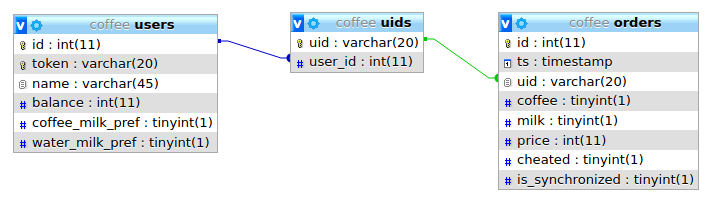
\includegraphics[width=16cm]{./images/database-diagram.png}
  % \captionsetup{justification=centering}
  \caption{Database schema for offline mode and milk preference.}
  \label{fig:db-scheme}
\end{figure}

\subsubsection{Storing the Milk Preference}
For the feature as described in \textbf{GUI03}, the assumption is made that a user habitually drinks their coffee either with or without milk.
This habit would only change rarely and the most probable cause would be that there is no milk left.
Currently, the milk preference is set after every order and, in consequence, just reflects the last choice made.
Thus, the simplest way to implement the feature would be retrieving the milk choice from the last order.
Nevertheless, the preference is stored separately in the users table in the local database (\autoref{fig:db-scheme}).
This leaves room for further improvement of the feature, maybe by adding a separate menu to change the preference.

Initially, it was assumed that users who drink coffee sometimes also take hot water to make tea and possibly want to drink it with milk.
Therefore, a milk preference for hot water was added.
Later this idea was dropped for three reasons:
1. Users were accustomed to make the milk choice before selecting a product on the coffee machine 
and it would not have been possible to pre-load the milk choice before the system knows if the user gets coffee or hot water;
2. There was no known user who drank their tea with milk;
3. Non trivial changes in the accounting server would have to be made to be able to register hot water with milk.
Nonetheless, the code and the database column for this feature were not removed.

\subsubsection{Entertainment Content}
Along with the new design of the GUI, the entertainment content feature was overhauled, also adressing \textbf{GUI04}.
While the system is in the state \texttt{get\_uid}, the user can view images for entertainment.
These images were only comics in V2 and now are complemented by a news feed in V3 .
Completely new are the ability to use two-finger swipe for zooming and panning the view,
and an automatic slideshow. A screenshot of the GUI displaying entertainment content can be found in the appendix \ref{sec:figures}.
The software will load any image, with a supported file extension, located in \texttt{./res/images/}.
After displaying an image for 90 seconds, the next image will be shown automatically.
The supported file extensions are \texttt{.jpg, .jpeg, .png, .gif}.
There is no support for animated GIFs.

To always display new content, images are downloaded from different services automatically.
In order to integrate better with the image viewing mechanism,
news articles are simply rendered from an RSS text feed into an image. 
A limit for the maximum number of images to keep from each service can be set.
All images beyond that limit will be deleted after an update, oldest first.
The system is kept simple to allow for easy extension with new services.


\subsubsection{Scheduler}
It is necessary to periodically synchronize offline orders, download images for entertainment content and afterwards reload the image viewer.
Therefore a simple scheduler was implemented. It is run in a separate thread, using only one single timer.
All registered tasks will be triggered by the same timer, every 3 hours.
A useful feature is to be able to pass a condition for the execution of the scheduled tasks. 
This makes it possible to only allow the scheduler to run a task when there is no order currently in progress,
avoiding additional load that could have a negative impact on the ordering process.

\subsubsection{Cheating Protection}
In V2 there were two ways of tricking the system into unlocking the machine without registering the order.
The first bug that can be exploited when refilling the water tank is already described as \textbf{BUG04}.
Rewriting the GPIO handling and IPC removed latencies that were causing this issue.

\textbf{BUG05} describes the second bug that a user could exploit to get free coffee. 
It was possible by ordering a coffee and then immediately pressing the cancel button in the GUI.
This is dealt with by saving the timestamp when a user logs in and then, if a \texttt{coffee\_ground} event occurs while in the state \texttt{get\_uid},
checking if the last login was within a time frame of 270 seconds.
The time frame is the sum of the current cancel timeout for logging the user out after 180 seconds, 
and a 90 seconds buffer where coffee could be ground.
If the last login was within that time frame, the user is logged in again and the system will proceed as with a normal order.
The only difference will be an additional note that will be sent to the accounting
server, documenting the cheating attempt.

\subsubsection{Code Quality}
While implementing new features and reorganizing code, 
special attention was directed to creating documentation
and writing clean code.
As a result, \textbf{F07} could be improved.

\subsection{An Improved Design for the 3D-Printed Case}
The first step in the design process is to create the model in Blender.
One has to keep in mind that, depending on the 3D printer's dimensions,
a model has to be sliced into several smaller parts to fit.
In this case it is three different parts.

For the new design the problems found in \textbf{BUG08} were fixed.
The thickness for all outside walls was set to 3mm uniformly.
This measure was found to result in a stable structure
that does neither break nor deform too easily. It also does not waste as much material.
The top part slides into the bottom part from the rear and is locked into place with a screw.
Little cylinders that fit exactly into the Raspberry Pi's screwing holes
are located on the floor of the bottom part.
The USB and LAN sockets fit exactly into the excavations in the rear side.
Together with the top part pushing down on the Raspberry Pi, the board is held in place without any additional screws.
A socket for screwing the RFID reader to the top part from below was added, too.
On the upper side of the top part the RFID symbol is engraved to show users where to place their RFID.
On the rear side of the top part there are openings for air circulation.
On the rear side of the bottom part there is one hole for the LAN cable and another 
opening where one part of the adapter board can fit through. 
After receiving user feedback about key chains with RFID chips attached falling down from the top,
a barrier was added around the top surface to prevent this from happening.
The final 3D model can be seen in \autoref{fig:new-case}.

\begin{figure}[h]
  \centering
  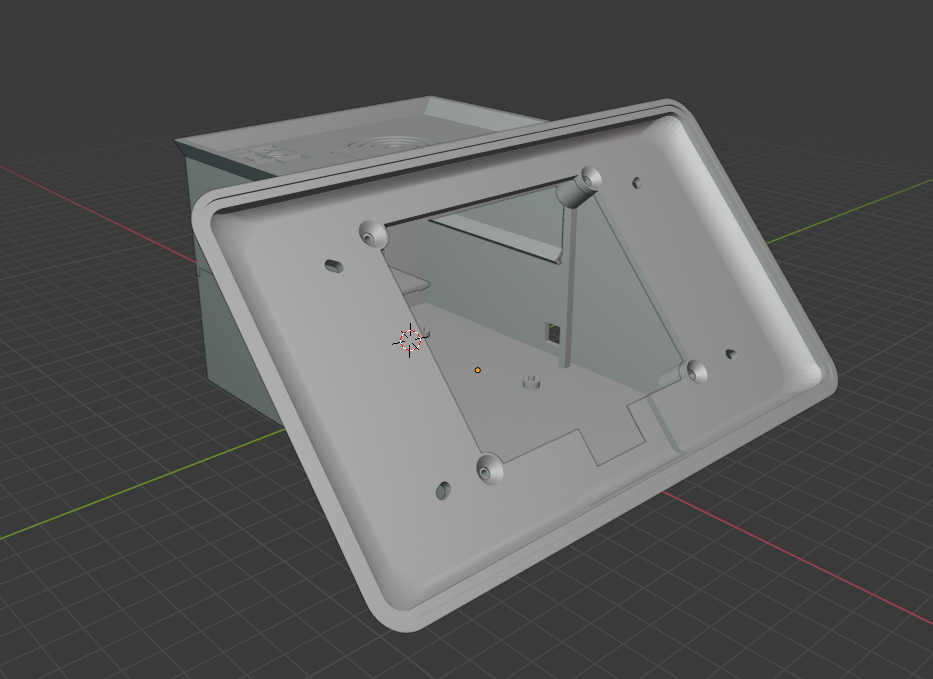
\includegraphics[trim={5cm 1cm 2.5cm 2.4cm},clip,width=0.49\textwidth]{./images/new-front.png}
  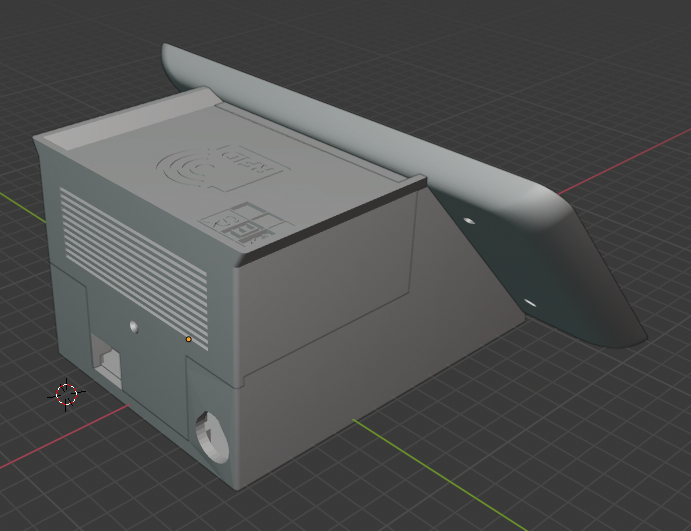
\includegraphics[trim={1cm 1cm 1cm 0cm},clip,width=0.5\textwidth]{./images/new-rear.png}
  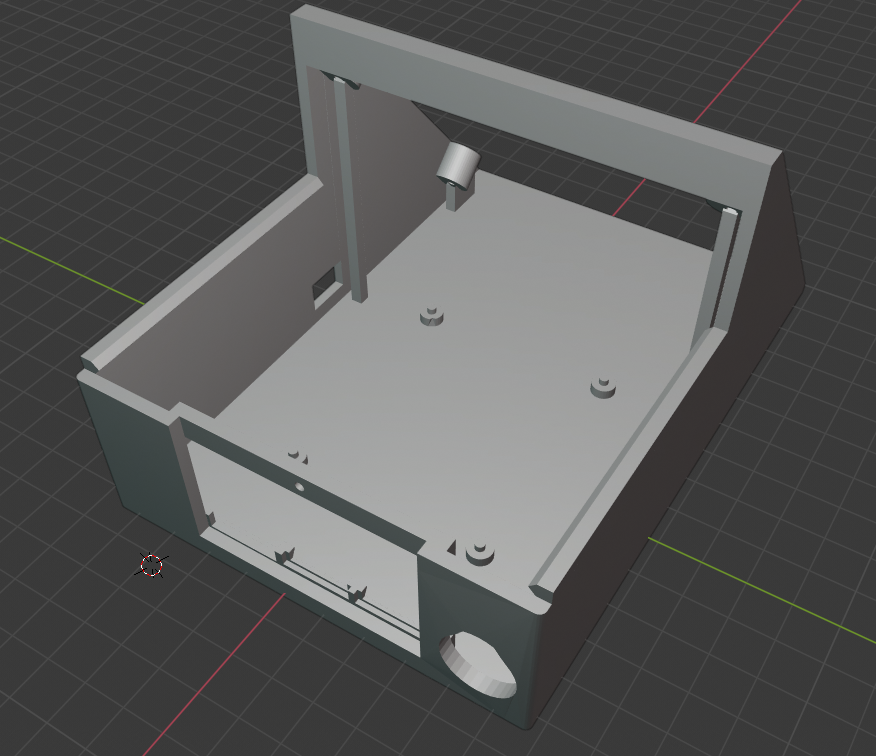
\includegraphics[width=0.49\textwidth]{./images/new-rear-bottom.png}
  \caption{The final 3D model of the case for V3.}
  \label{fig:new-case}
\end{figure}

Once the model has the desired shape, the mesh has to be cleaned up and checked for errors.
In Blender 2.8+ this is done by selecting ``Mesh $>$ Clean Up $>$ Merge by Distance", ``Mesh $>$ Clean Up $>$ Delete Loose" and ``Mesh $>$ Normals $>$ Recalculate Outside".
These commands will remove obsolete geometry and recalculate the inside and outside of the mesh.
The check that follows afterwards is the most important one, as it checks for solidity.
The most common problem is non-manifold geometry, 
internal faces, areas with no thickness or disconnected vertices,
as these make it impossible to calculate the models volume unambiguously.
In initial iterations of the design process, the model appeared to be solid, when in fact it was not.
This led to parts not being connected, components falling apart and walls being hollow and filled with uncured resin.
Therefore, the ``3D-Print Toolbox" add-on has to be used to analyze the mesh for potential problems.
The tool will highlight ambiguous geometry that has to be corrected manually most of the times.

The next step consists of exporting the model from Blender and importing it into formlab's \textit{PreForm} tool
using the STL file format. The vendors software can automatically repair a few problems in the model if they are not too grave.
A preview of the model is shown and it has to be processed for printing.
Supporting structures are added automatically to prevent overhanging parts from falling. This can be seen in \autoref{fig:preform}
The structures can be removed after printing. 
However, they will cause a bumpy surface on planes that they are attached to.
In consequence, when placing the structures, which is done implicitly by changing the models orientation,
less visible contact surfaces should be preferred.
Ideally, supporting structures are not attached to small parts that could accidentally be torn of when removing the structures.
The models orientation directly influences the amount of structures, material and printing time needed.
It is a good practice to experiment with different orientations to preview the calculated supporting structures and material requirements.

\begin{figure}[H]
\centering
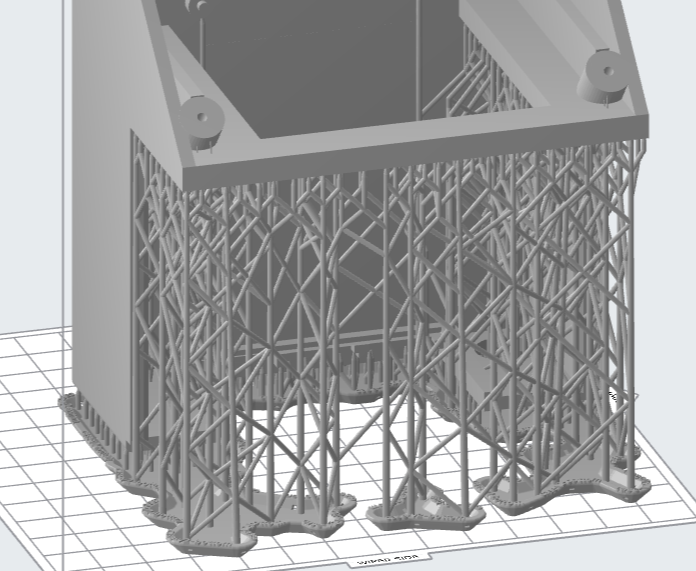
\includegraphics[width=0.39\textwidth]{./images/bottom-preform.png}
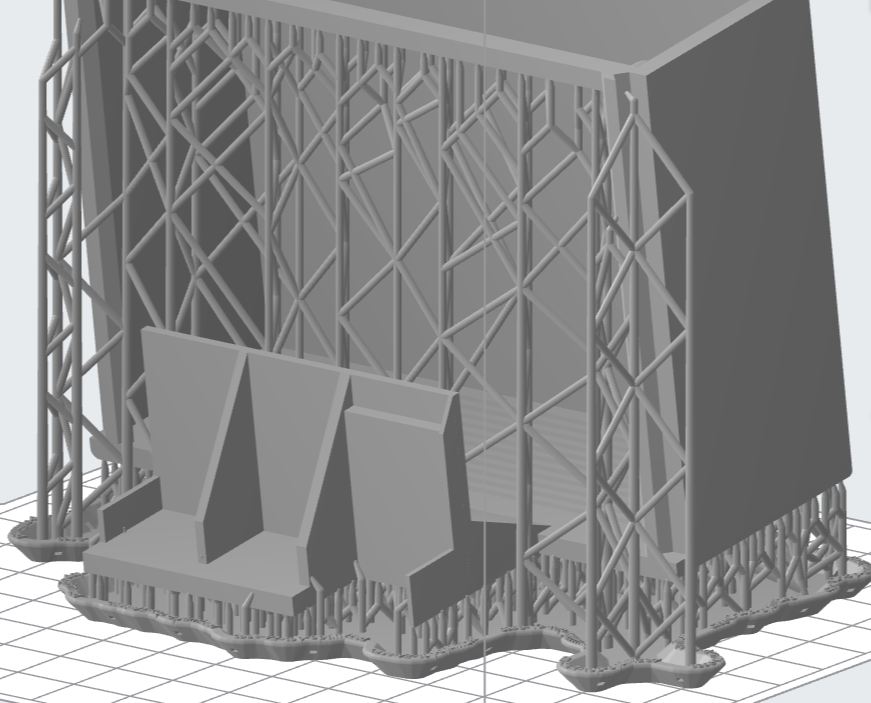
\includegraphics[width=0.4\textwidth]{./images/top-preform.png}
\caption{3D models of top and bottom part with supporting structures.}
\label{fig:preform}
\end{figure}


\section{Results}

\subsection{Improvement of Usability and Reliability}
Measuring the improvement of usability can be difficult to put in numbers.
In theory usage studies would be performed, interviewing every user or letting them fill out a questionnaire.
However, in this environment it would be impractical to perform a study like this.
In consequence, the improvement of usability is only measured in terms of changes made
to reflect the requirements for usability that were examined in \autoref{sec:usability}.
Out of the 21 problems and shortcomings listed in \autoref{pa:list},
only 3 are not directly related to usability considerations.
These three problems are F02, F04 and F07; CPU usage, logging and code quality.
More importantly, the remaining part of issues that had negative effects on usability was resolved, 
leading to a significant improvement.

Furthermore, it can be argued that because of the iterative evaluation of design changes
and the integration of user feedback during the development process,
usability and overall user satisfaction with the system were naturally improved.

The close link between usability and reliability was explained in the introduction.
By resolving the bugs that caused the system to crash or freeze,
an improvement of reliability was accomplished.

A common practice of users was to unplug and plug the Raspberry Pi from power, in order to restart the device.
These manual restarts are a good indicator for software faults.
Since deploying V3 these events were perceived to occur less frequently than it was the case with V2,
to a point, where the device was even observed to run for one complete month without restart.
Unfortunately, with the scarce data available from V2 it was not possible to proof this hypothesis.
To measure the improvement of reliability in numbers, long term statistics from V2 would be required.

Although informal and hard to quantify, it should be mentioned that users said they were able to rely on the system again
in a way that they could be sure they can use it any time they want, without running into problems. 
Also it is worth to mention that the consecutive uptime of the system in V3 significantly increased when compared to V2,
which indicates that there was no need for manually restarting the system when in an error state.
However, no guarantees can be made for a certain availability.

\subsection{Improvement of Performance}
To measure and compare the performance of both versions, the system was rebooted and then it ran for one hour before the
statistics were retrieved with the Unix command \texttt{ps axo pcpu,pmem,args}.
During the time of measurement no orders were taken.
The results can be seen in \autoref{tab:perf-v2} and \autoref{tab:perf-v3}.
It is easy to conlude that the changes made in \ref{sec:cpu-usage} to improve the CPU usage were effective. 
While in V2 CPU usage for the GPIO and buzzer functionality alone was at 98.1\%,
it dropped to a cumulated value of 6.3\% in V3.
For V3 the CPU usage of the pigpio daemon (pigpiod) has to be added to the CPU usage of the actual process for handling GPIO.

  \begin{table}[H]
  \centering
  \begin{tabular}{lllr}
   \hline
  \% CPU & \% memory & python module\\ 
  \hline
  98.1 & 1.8  & inputGPIO.py (GPIO \& buzzer)\\
  12.4 & 2.1  & inputGPIO.py (RFID)\\
  0.1  & 10.2 & main.py (GUI)\\
  0.0  & 1.6  & inputGPIO.py (locking)\\
  \hline
  \end{tabular}
  \caption{Performance measurements of version V2, one hour after boot.}
  \label{tab:perf-v2}
  \end{table}
  
  \begin{table}[H]
  \centering
  \begin{tabular}{lllr}
   \hline
  \% CPU & \% memory & python module\\ 
  \hline
  5.9  & 0.1  & pigpiod (GPIO)\\
  16.3 & 3.9  & main.py (RFID)\\  
  0.7  & 10.6 & main.py (GUI)\\
  0.4  & 4.6  & main.py (GPIO \& locking)\\
  0.0  & 4.4  & main.py (buzzer)\\
  \hline
  \end{tabular}
  \caption{Performance measurements of version V3, one hour after boot.}
  \label{tab:perf-v3}
  \end{table}

\% CPU is the ``cpu utilization of the process in "\#\#.\#" format.
Currently, it is the CPU time used divided by the time the process has been running (cputime/realtime ratio),
expressed as a percentage.", and 
\% memory is the ``ratio of the process's resident set size  to the
                             physical memory on the machine, expressed as a
                             percentage." \cite{MAN:ps}.


\subsection{3D Printing Cost Calculation}
In the end, the amount of resin needed for the final 3D model printed were:
For the top part, volume without support structures 65.63ml, total volume 90,79ml.
For the bottom part, volume without support structures 96.88ml, total volume 150.08ml.

The Form 2 Resin Tank is sold for €65.45 and has to be replaced after a printing volume of 1-1.5 liters.
1 liter of the Grey Resin\footnote{Product number: RS-F2-GPGR-04}, which was the type of resin used, costs €160.65.
These are the prices from the manufacturer's online shop plus german VAT.
A conservative cost calculation for printing would be:
\[\frac{\text{€}65.45 + \text{€}160.65}{1000 ml} = \text{€}0.2261/ml\]
With the cost per ml the costs for the different parts can be calculated:
\begin{itemize}
  \item The top part, with a volume of 90.79ml, costs €20,53.
  \item The bottom part, with a volume of 150.08ml, costs €33.93.
  \item The screen frame, with a volume 53.60ml+\footnote{For the screen frame only the volume without supporting structures is available, as it was already printed for V2.}, costs €12.12.
\end{itemize}
This results in a total of €66.58 in printing costs for the final model.
Taking into account all the failed printing attempts during development of the model,
including the models for V2, the total material cost could be estimated to lie above €300.

\section{Conclusion}
In the introduction the goal of this thesis was outlined as documenting the improvement of V2's usability and reliability.
The design and implementation changes with the greatest positive impact on these two aspects are:
\begin{itemize}
  \item Controlling core logic with the FSM, as it simplifies reasoning about control flow;
  \item Using interrupts instead of polling for GPIO, as it greatly reduces processor usage and, as a result, power consumption;
  \item Having a more user-friendly design for the GUI, as it makes usage of the device easier and simplifies first-time use;
  \item Finishing the 3D printed case, as it gives the whole appliance a more elegant and satisfying look in comparison the shoe box from before.
\end{itemize}

To evaluate the different design choices made,
feedback from the users was gathered during daily usage
and later utilized to optimize the design in several iterations.
Throughout the thesis, the importance of usability during the design process was illustrated,
showing that by following usability guidelines the final product can be improved significantly.
Especially in the context of IoT technologie this point is crucial and, in the opinion of the author,
still neglected by many.
Ultimately, it can be confidently concluded that the final system
has now reached a point were it absolutely is an advantage over using a paper tally sheet
and even more so with the strong focus on usability.

\section{Future Work}
Debugging the hardware to find what is causing the coffee grinder signal not to be recognized 
should be considered the most important topic to work on.
The workaround that was created for V3, does prevent financial loss, but otherwise is not very satisfying.

Another category of features could be implementing more warnings in the GUI for people with undesirable behavior,
such as the ``bad milk guys'' or people who leave it to the next person to refill the water tank.
For a greater effect, an alarm sound could be played with the buzzer, once a certain warning is displayed.
Additionally, these warnings could be sent out automatically to every user's email address.

Because the system is switched on 24/7,
it is not ideal that the screensaver is currently deactivated permanently.
A screensaver that only gets enabled outside of the normal usage hours,
and only if the water tank is not currently empty, could be developed.
Ideally, the screensaver would be disabled by touching the screen.

To take the idea of saving power a step further,
the Raspberry Pi could be equipped with a relais for 330VAC power to control the coffee machine. 
Like that, the coffee machine could be switched off completely at night hours,
only switching on when required. This might also make it possible to control the coffee machine's heating.
Another interesting feature to improve usability and save time could evolve out of this.
Users could have the possibility to go on a website served by the accounting server and initiate the heating of the coffee machine
before they go to the room where the coffee machine is located.

\pagebreak
\begingroup
\pagestyle{empty}
\null
\newpage
\endgroup

%------------------------- Literaturverzeichnis ---------------------------- 
\bibliographystyle{alpha}
\bibliography{ausarbeitung.bib}

\pagebreak
\clearpage
\begingroup
\pagestyle{empty}
\null
\newpage
\endgroup

\appendix
\section{Appendix}
\subsection{Settings}
The system has to be restarted after making any changes described here.
Use \texttt{sudo systemctl restart coffee-v3}
\subsubsection{How to Change Prices}
It is not sufficient to change prices in the accounting server's database.
Price updates are not automatically fetched by the system, because they do not occur frequently enough.
To change the prices, the values of the according constants in \texttt{order.py} have to be adjusted.

\subsubsection{How to Change Dispensing Limit}
\label{app:dispensing}
To change the thresholds, which the user's balance has to fall below before 
\begin{enumerate}
  \item a warning about the account being locked is shown and 
  \item the account is locked,
\end{enumerate}
adjust the constants \texttt{DISPENSING\_WARN} and \texttt{DISPENSING\_DENY} in \texttt{main.py}.
Both positive and negative values are allowed.
However, \texttt{DISPENSING\_WARN} should always have a greater value than \texttt{DISPENSING\_DENY}.

\subsubsection{How to Change Admin Passcode}
The source code for the admin login can be found in \texttt{src/gui/admin\_login.py}.
There the passcode is stored in the variable \texttt{self.password} and can be changed to any series of numbers.

\subsection{Raspberry Pi 3 Model B V1.2 Specifications}
\label{PI:Spec}
\begin{itemize}
  \item Broadcom BCM2837, quadcore Cortex-A53 (ARMv8) 64-bit SoC @ 1.2GHz
  \item 1GB LPDDR2 SDRAM
  \item BCM43438 wireless LAN and Bluetooth Low Energy (BLE) on board
  \item 100 Base Ethernet
  \item Extended 40-pin GPIO header
  \item 4 USB 2 ports
  \item 4 Pole stereo output and composite video port
  \item Full size HDMI
  \item CSI camera port for connecting a Raspberry Pi camera
  \item DSI display port for connecting a Raspberry Pi touchscreen display
  \item Micro SD port for loading your operating system and storing data
  \item 5V/2.5A DC power input
\end{itemize}

\subsection{System configuration}
\subsubsection{Systemd Service}
\label{systemd-service}
\begin{figure}[H]
  \lstinputlisting[basicstyle=\footnotesize,frame=single]{../coffee-v3/systemd/coffee-v3.service}
  \caption{The configuration file for the systemd service.}
\end{figure}

\subsubsection{Security}
The Raspberry Pi has a static and publicly accessible IPv4-Address.
It is a so called exposed host, not protected by a network firewall.
To lower the risk of unauthorized access, the following measures were taken:
\textit{fail2ban} bans ips that fail to authenticate with ssh several times in a row.
\textit{iptables} were configured to only accept connections from inside KIT-Network and drop all other connections.
\textit{unattended-upgrades} is used to automatically install security updates.

\subsection{Accounting Server}
\subsubsection{Fixing Problems after Update}
The statistics diagram on the accounting server's website stopped working properly.
This was related to an operating system upgrade on the server which updated php and mysql versions.

The new version of php is 7.2. It was php5.* before.
Statements had to be replaced as follows to run the code without errors:
\begin{lstlisting}{language=php}
    # pre php7
    mysqli_escape_string($string)
    
    # php7
    mysqli_escape_string($link, $string)
  \end{lstlisting}

The new version of the MySQL DBMS is 5.7.28, before it was below 5.7.5.
MySQL 5.7.5 and newer activate the ONLY\_FULL\_GROUP\_BY mode by default.
In this mode all queries are checked for functional dependence.
MySQL rejects queries for which the select list, HAVING condition,
or ORDER BY list refer to nonaggregated columns that are
neither named in the GROUP BY clause nor are functionally dependent on them.

\subsubsection{Repairing Order Log on Accounting Server}
There was a bug in the new software that caused all orders to be processed as ``Coffee with Milk". This condition lasted about one month before it was detected and fixed.
During that time users were charged more money for their black coffees and hot waters. Luckily, there is a local copy of the orders on the Raspberry Pi. This could be used to repair the false data.
First the data in the affected time period were extracted from the databases. Then a Python script was used to merge the data and create an SQL query for every corresponding database row.

\begin{lstlisting}{language=sql}
    # accounting server database
    SELECT * FROM coffee.protokoll WHERE id >= 20643 AND id <= 20974 AND Kommentar LIKE '%rfid%' AND UserID != 124;

    # local database 
    SELECT * FROM coffee.orders where id >= 10 and id <= 277 and uid != 0123;
\end{lstlisting}

Ultimately, after performing a database backup via the \texttt{mysqldump} CLI tool, the generated sql update statements were applied to the accounting server database.

\begin{lstlisting}{language=sql}
      SET sql\_mode=(SELECT REPLACE(@@sql\_mode,'ONLY\_FULL\_GROUP\_BY',''));
\end{lstlisting}

\subsection{Figures}
\label{sec:figures}
\begin{figure}[H]
\centering
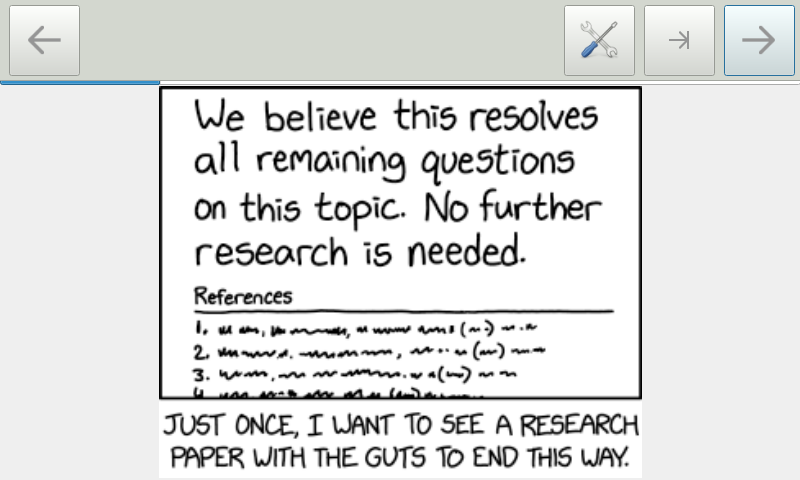
\includegraphics[width=\textwidth]{./images/entertainment.png}
\caption{Entertainment content in the GUI.}
\end{figure}
\end{document}
